%\documentclass[natbib,preprint]{sigplanconf}
% \documentclass[conference]{IEEEtran}
\documentclass{sig-alternate}
\usepackage{fancybox}
\usepackage{cite}
\usepackage{color,soul}
\usepackage{hyperref}
\usepackage{algorithmic}
\usepackage{flushend}
\usepackage{fancyvrb}
\usepackage[normalem]{ulem}
\usepackage{graphicx}
\usepackage[lined, algonl, ruled, boxed]{algorithm2e} 
\usepackage{amsmath}
\usepackage{amssymb} 
\usepackage{graphicx}
\usepackage{verbatim}
\usepackage{booktabs}
\usepackage{multirow}
\usepackage{listings}
\usepackage{subfigure}
\usepackage{latexsym}
\usepackage{xspace}
\usepackage[usenames,dvipsnames]{xcolor}

% \usepackage{fancybox}
% \usepackage[usenames,dvipsnames,svgnames,table]{xcolor}
% \captionsetup[table]{skip=10pt}

\newcommand{\tool}{\textsc{Clipboard}\xspace}
\newcommand{\fixme} [1] {\textcolor{red}{{\it FIXME}: #1}}
\newcommand{\delete} [1] {\textcolor{red}{#1}}
\newcommand{\add} [1] {\textcolor{blue}{#1}}
% \newcommand{\javac}{javac\xspace} % This package lets you punctuate \javac normally and get good spacing, e.g., \javac.  gives you: javac.
\newcommand{\codefont}[1]{\footnotesize{\texttt{#1}}\normalsize}
\newcommand{\todo} [1]{\textcolor{blue}{{\sf TODO}: #1}}
\newcommand{\hlc}[2][yellow]{ {\sethlcolor{#1} \hl{#2}} }


% \lstset{frame=tb,
%   language=Java,
%   showstringspaces=false,
%   columns=flexible,
%   basicstyle={\ttfamily\footnotesize},
%   numberstyle=\tiny\color{gray},
%   keywordstyle=\color{blue},
%   commentstyle=\color{dkgreen},
%   stringstyle=\color{mauve},
%   breaklines=true,
%   breakatwhitespace=true,
%   tabsize=3
% }



\begin{document}

%\conferenceinfo{Mystery'09,} {January 1, 2009, Austin, TX.}
%\CopyrightYear{2009}
%\copyrightdata{2009}


%\title{How Universal are Naming Rules?}

\title{Weekly Meeting 10/6/2015} %
\subtitle{Focus on Problem 2, find examples to prove this problem}
% \numberofauthors{3} 
% \author{
% You can go ahead and credit any number of authors here,
% e.g. one 'row of three' or two rows (consisting of one row of three
% and a second row of one, two or three).
%
% The command \alignauthor (no curly braces needed) should
% precede each author name, affiliation/snail-mail address and
% e-mail address. Additionally, tag each line of
% affiliation/address with \affaddr, and tag the
% e-mail address with \email.
%

\numberofauthors{1} %  in this sample file, there are a *total*
% of EIGHT authors. SIX appear on the 'first-page' (for formatting
% reasons) and the remaining two appear in the \additionalauthors section.
%
%\author{
% You can go ahead and credit any number of authors here,
% e.g. one 'row of three' or two rows (consisting of one row of three
% and a second row of one, two or three).
%
% The command \alignauthor (no curly braces needed) should
% precede each author name, affiliation/snail-mail address and
% e-mail address. Additionally, tag each line of
% affiliation/address with \affaddr, and tag the
% e-mail address with \email.
%
% 1st. author
%\alignauthor
%Lisa Hua$^{\dag}$ Na Meng$^{\dag}$ Miryung Kim$^{\ast}$ Kathryn S. McKinley$^{\ddag}$\\
%\affaddr{$^{\dag}$\normalsize{The University of Texas at Austin~~~~~~~$^{\ast}$University of California, Los Angeles~~~~~~~$^{\ddag}$Microsoft Research}}\\
%\email{\normalsize{\{lisahua@, mengna09@cs\}.utexas.edu, miryung@cs.ucla.edu, mckinley@microsoft.com}}
%}

\maketitle


\section{Problem}  
To obtain necessary functionality, developers often use third-party libraries. Due to the complexity of current software systems, the dependency issue arises when the system depend on different and incompatible versions of the same library. This issue, called  `dependency hell'~\cite{wiki:hell} may break other dependencies or push the problem to another set of libraries. When developers try to introduce a new library or upgrade existing ones, then other applications on their system might suddenly break as the newly-introduced libraries are not backward-compatible to the existing libraries. We use an example to illustrate how the `dependency hell' causes a build error, how it is localized, how it is fixed in the next session. 

%\noindent{\bf{Problem }}

\section{Example}


 \begin{figure}[!htb]
 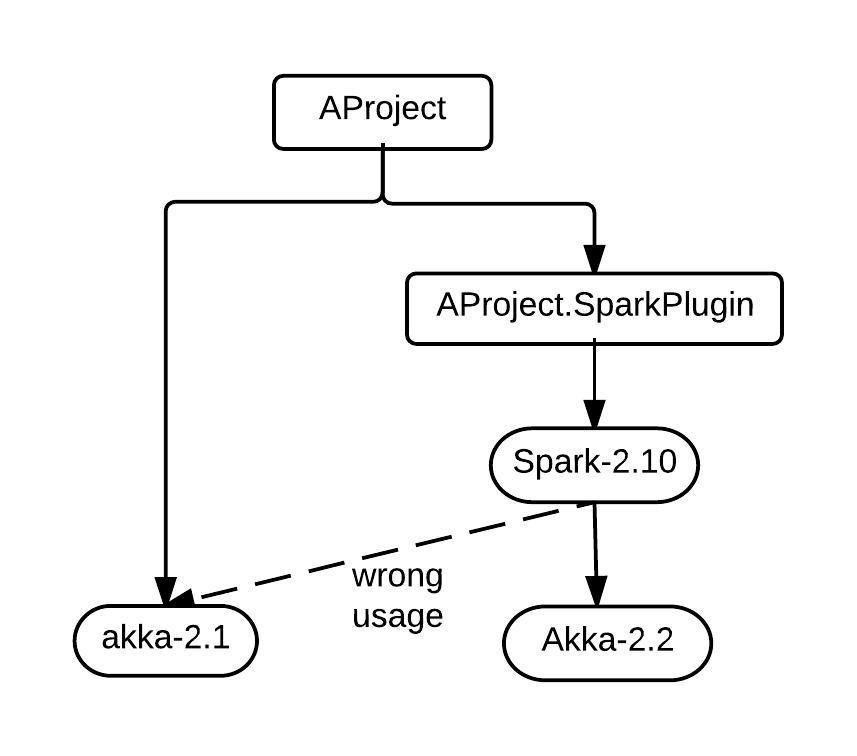
\includegraphics{akka.jpeg}
 \end{figure}
\noindent{\bf{What is the `dependency hell'?}}

\begin{figure}[!htb]
 \begin{minipage}{0.47\textwidth}
\scriptsize 
\begin{tabular}{@{}p{1\textwidth}} 
 \hline 
%  \multicolumn{1}{c}{(A) An inconsistent object name found by both Lancelot and \tool } \\ \hline
%  \vspace{-4mm}
%\begin{Verbatim}[commandchars=\\\{\}, tabsize=2]
% /* org.elasticsearch.action.DeleteRepositoryRequestBuilder */
%1.public String setName() \{
%2.  return setName;
%3.\}
%\end{Verbatim}
%\vspace{-4mm}
% \\ \hline
  \multicolumn{1}{c}{(A) Methods queried by user} \\ \hline
    \vspace{-4mm}
\begin{Verbatim}[commandchars=\\\{\}, tabsize=2]
/* org.apache.jena.json.JsonWriter */
1. public class JsonWriter implements JsonVisitor \{
2.  OutputStreamWriter writer;
3.  public void \bf{visit(JsonNumber jsonNumber)}  \{
4.   print(jsonNumber.value()) ; 
5.  \}
6.  public void \bf{visit(JsonBoolean jsonBoolean)} \{
7.   String x = Boolean.valueOf(jsonBoolean.value())?"true":"false"; 
8.   print(x);
9.  \}
10. private void \underline{print(Object s)} \{...
11.  writer.println(s);
12. \} ...\}
 \end{Verbatim}
   \vspace{-4mm}
  \\ \hline
   \multicolumn{1}{c}{(B) Callers of these two methods} \\ \hline
  \vspace{-4mm}
\begin{Verbatim}[commandchars=\\\{\}, tabsize=2]
 /* org.apache.accumulo.core.sync.SortedMapIterator */
1. public class JsonNumber extends JsonValue \{
2.  Format format;
3.  @Override
4.  public Object \underline{value()}
5.   \{ return format.getValue(value); \}
6.  @Override
7.  public void \uwave{visit(JsonVisitor visitor)}
8.   \{ visitor.visit(this) ; \}
9. \}
10. public class JsonBoolean extends JsonValue \{
11.  @Override
12.  public Object \underline{value()}
13.   \{ return value; \}
14.  @Override
15.  public void \uwave{visit(JsonVisitor visitor)}
16.   \{ visitor.visit(this) ; \}
17. \}
 /* Three of other 13 callers */
18. public class JsonFormatNumberHandler extends JsonHandler \{
19.  public static void \uwave{printNumber(JsonNumber jNum)} \{
20.   JsonWriter w = new JsonWriter(output);
21.   jNum.setFormat(format);
22.   w.visit(jNum);
23. \} ...\}
24. public class JSONNumberOptional \{
25.  JsonBoolean jBool; 
26.  JsonNumber left, right;
27.  public static void \uwave{recordOptional()} \{
28.   JsonWriter w = new JsonWriter(output);
29.   w.visit(left);
30.   w.visit(jBool);
31.   w.visit(right);
32. \} ...\}
33. public class JSON \{
34.  public static void \uwave{write(JsonValue jValue)} \{
35.   JsonWriter w = new JsonWriter(output);
36.   w.visit(jValue);
37. \} ...\}
\end{Verbatim}
\vspace{-4mm}
 \\ \hline
\end{tabular} 
\caption{Example of suggested elements given a set of interest}
\label{fig:compare}
\end{minipage}
\end{figure}



%%%%%%%Usage pattern example %%%%%%%

%
%\begin{figure}[!htb]
% \begin{minipage}{0.47\textwidth}
%\scriptsize 
%\begin{tabular}{@{}p{1\textwidth}} 
% \hline 
% \multicolumn{1}{c}{(A) An inconsistent object name found by both Lancelot and \tool } \\ \hline
%  \vspace{-4mm}
%\begin{Verbatim}[commandchars=\\\{\}, tabsize=2]
% /* org.elasticsearch.action.delete.DeleteRepositoryRequestBuilder */
%1.public String setName() \{
%2.  return setName;
%3.\}
%\end{Verbatim}
%\vspace{-4mm}
% \\ \hline
%  \multicolumn{1}{c}{(B) A naming bug from Lancelot} \\ \hline
%   \vspace{-4mm}
%\begin{Verbatim}[commandchars=\\\{\}, tabsize=2]
%/* org.elasticsearch.action.termvector.TermVectorFields */
%1.public void size(int size) \{
%2.  if (size <= 0) 
%3.   throw new legalArgumentException("Size must be positive"); 
%4.  this.size = size;
%5.\}
% \end{Verbatim}
% Lancelot said: Methods with this name never return void.
% \vspace{-4mm}
%  \\ \hline
%\end{tabular} 
%\caption{Name Checker comparison}
%\label{fig:compare}
%\end{minipage}
%\end{figure}
 

We illustrate the building error caused by `dependency hell' in a Maven project shown in Figure~\ref{fig:shifu}. As shown in part A, the parent project uses akka 2.1.1 to initialize \codefont{ActorRef} (underline) by creating a new \codefont{Props} object. The developer Alice is asked to implement a new sub-module named as SparkPlugin using Spark framework. Without knowing that Spark is dependent on akka-2.2.3, she implements the entire sub-module with Spark-1.0.0, writes the tests, and fully tests the single submodule before integrating with the parent project. However, she encounters the building error shown as part (C) (The complete building error is shown at~\cite{shifu}). 

\noindent{\bf{How to localize `dependency hell'?}} 

Starting from the \codefont{NoSuchMethodException}, she investigates the \codefont{akka.remote.RemoteActorRefProvider.<init>}  in akka-2.2.3 as declared in Spark's pom.xml and finds the static \codefont{Props.create} method shown in part (D). Alice get confused on the \codefont{NoSuchMethodException} and she has to use step-by-step debugging. She finally notices that the maven build system mistakenly uses akka-2.1.1 inherited from parent project, rather than the akka-2.2.3 that is required for Spark library. 

\noindent{\bf{How to fix `dependency hell'?}}

  Alice has several options to fix this bug as below:
\begin{enumerate}
\item change akka version in parent class to 2.2+, which is not feasible as the parent project heavily uses akka and it requires tremendous effort for upgrading.
\item  exclude all transitive dependencies inherited from parent project with the feature provided by Maven 3.2.2+~\cite{maven:note}, aiming to resolve dependency hell~\cite{maven:hell}. This approach is not feasible as well because SparkPlugin itself relies on the parent projects and Alice has to re-import all dependencies that the submodule uses.
\item include both akka versions and enforce Spark to use akka-2.2.3. This approach is similar to the well-known side-by-side  mechanism used in NIX package manager for Linux-based system~\cite{nix}. This might fix the build error, but Alice is concerned that compiling both versions might increase the building time of the entire system. 
\item exclude akka-2.1.1 from the dependency declaration of Spark-1.0.0. Alice decides to use this solution as it won't have ripple effect on the rest of the system.
\end{enumerate}


%To ensure that there does not exist any other transitive dependency that causes dependency hell, she tries maven-enforcer plugin which have the rule to ban all transitive dependencies~\cite{maven:enforcer}, yet the plugin outputs more than 100 conflicts. Alice gives up to kill all conflicts as (1) It is costly to exclude all conflicts, (2) it makes the maven hard to maintain, and (3) most of them might not be harmful for the system. 

Using this example, we illustrate that  it is not easy to  localize dependency hell without knowing the entire dependency graph and it can be error-prone when trying to fix the error.

\section{Related Work}

When two versions of the same library occur, Maven selects the closest library  in the tree of dependencies by default~\cite{maven:depend} (e.g., if dependencies for A, B, and C are defined as A -> B -> C -> D 2.0 and A -> E -> D 1.0, then D 1.0 will be used when building A because the path from A to D through E is shorter). User is able to manually exclude or force Maven to use a specific version, but the correctness is not guaranteed~\cite{maven:note}. Maven Enforcer Plugin checks a set of build rules including a Ban-Transitive-Dependency rule that detects all transitive dependencies conflicts and force users to resolve all conflicts. The Enforcer Plugin only checks the \codefont{groupid}, \codefont{artifactid}, and \codefont{version} declared in the configuration file (\todo{Lisa: though I don't know if we need to check semantics or compatibility of different versions, I leave this limitation for future reference}), and it does not help developers fix the conflicts without breaking any other parts of the system.
The majority of existing build systems model dependencies identical to Maven. Examples include Gradle, MSBuild, Make, and CloudMake. The features that make them different are unrelated to dependency management, but on syntax of build scripts and parallelization. 

Bazel is a new build system developed by Google that advertises parallelization and correctness~\cite{bazel:depend}. Bazel does not allow transitive dependency and only reads dependencies listed in from the root dependency declaration file. This means that if your project (A) depends on another project (B) which list a dependency on project C in its WORKSPACE file, both transitive dependencies from B and C should be added to the WORKSPACE file. This can balloon the file size, but hopefully limits the chances of having one library include C at version 1.0 and another include C at 2.0. But they also assume that users can provide correct configuration and select correct versions of libraries. 

Package managers in operating system also encounter similar dependency management problem. To deal with destructive upgrade and multi-distribution support in Linux products, Nix ~\cite{nix} provides a co-existing package management mechanism to store a source package in its own directory, instead of a global location that share across the entire system. However, this might not work in build system like Maven, as with transitive dependencies, the graph of included libraries can quickly grow quite large~\cite{maven:depend}. 

\section{Approach}

%There are some well-known solutions to this problem, they either ask developers to manually exclude all the transitive dependencies for a dependency (Solution 2) or include multiple versions in a side-by-side manner (Solution 3). Neither of them are perfect as described in the previous session. 

%We propose an approach to verify the safety of upgrading and 

%We propose an approach to check compatibility on the interfaces that use different versions for the same libraries, which has the possibility to introduce `dependency hell'. Instead of strict backward compatibility checker for the entire class~\cite{Welsch:backward12}, we regard it as safe if the used API is compatible for the other version in the current usage context. We make this trade-off because developers often embrace changes, making multiple versions incompatible to each other~\cite{bogart:backward}. To save build time and space,  we include multiple versions of the files from the same library only if they are incompatible with each other, instead of maintaining multiple versions for the same library at the same time. To save time for analysis, we only consider the API calls when it has the possibility to generate `dependency hell', since there is no need to check the dependency issue if the libraries are consistent used in the system with a single version.



\section{Motivating Example}

Consider a reuse task to implement a drag-and-drop plugin called \tool for Eclipse to support systematic editing~\cite{Meng:sydit11}. As shown in Figure~\ref{fig:clipboard}, users drag and drop the method they want to edit to \tool before editing. When they finish changing the method, they take another snapshot using drag-and-drop. \tool will automatically recommend locations that  are similar to the given example, and recommend similar but not identical edits based on similar context. 

To complete this task, developer first queries Google code search (GCS) using the query \codefont{Eclipse plugin drag and drop to table}. We choose GCS because existing code example recommendation tools like Strathcona~\cite{Holmes:structural05} and code query tools like SNIFF~\cite{sniff:Sen09}  do not fit for such a medium scale reuse task. GCS returns 102 examples. We only analyze the first five returned examples because empirical evidence indicates that developers rarely look beyond this limit when searching~\cite{Starke:searchNum09}. The fourth example is much too long (over 1000 lines) without any explanation and the third and fifth example are duplicated with the first one. Figure~\ref{fig:dndweb} illustrates a snapshot for the first example returned by GCS. It implements a SWT shopping cart application to select items from all grocery items and put them into `My shopping cart' via drag-and-drop (Figure~\ref{fig:cartTable}). The second example implements an example for TODO labels which enables user to drag a TODO label from Editor Panel and drop it in an Eclipse Plugin List View (Figure~\ref{fig:todoList}). This is very similar to the task that requires to drag the source code from Editor Panel to an Eclipse Plugin View, yet we hope to use the table view to record multiple examples for both old version and new version, which is the format used in the first example. 

Our next step is to extract common API calls for drag-and-drop action. It is always hard to distinguish the main functionality and variants via a single example, but with the help of multiple examples, our tool is able to identify the main API calls that provide desired functionality. In this example, we notice that the main API calls will be \{new Viewer(), setTransfer(), setOperation(), addDragSupport(), addDropSupport()\} given the hierarchical fact that both \codefont{TableViewer} and \codefont{ListViewer} are subclasses of \codefont{Viewer}. 

After identifying the main API calls (and corresponding control structure), we investigate related elements for these API calls. The implementation of \{DropTargetListener, DragSourceListener\} are identified as common coupling elements, while \{TodoModelProvider, TableItem, GridLayout\} are excluded as they do not have corresponding mapping in the other example. We notice that we should override \{DropTargetListener.drop(), DragSourceListener. 

\noindent{dragSetData()\} to help us finish the drag-and-drop reuse task.}




\section{Approach}

To identify methods that implement concerns, I build a prototype which invokes Code Search Engine (CSE) API and analyzes the results from CSE using partial program analysis~\cite{partialProgram:OOPSLA08}. I select SearchCode~\cite{SearchCode} because it is an open source code search engine with over 7000 projects from  Github, Bitbucket, Google Code, and Sourceforge, with complete API documentations. To identify queried features in the returned source code,  I use the mean of TF-IDF weight  for each query term as a weighting factor and select top k (k=5) methods that are related to the given query.  This approach is similar to prior works that use  IR~\cite{Denys:FCA12} and NL analysis~\cite{Hill:FindConcept07} for feature location. I choose IR approach because other approaches require history or structural analysis that might not be feasible for partial program. TF-IDF =  $avg( \log (1 + f_{t,d}) \times  \log \frac {N} {n_t}), f_{t,d}$ is the frequency of term $t$ in method $d$, $N$ is the total number of methods, $n_t$ is the number of methods that have the term $t$.

\section{Related Work}

\paragraph{Corpus-wide Naming Rules}  Abebe et al.\/ investigate identifier quality  based on a catalog of Lexicon Bad Smells~\cite{abebe:wcre12}. 
Caprile and Tonella leverage pre-defined syntax and identifier dictionary to replace terms with their synonyms to ensure naming consistency~\cite{caprile:reconstruct}. Dei{\ss}enb{\"{o}}ck and Pizka proposed a formal model for concise and consistent naming, which requires a mapping from a concept domain to a lexical domain~\cite{ccnames:Pizka06}. Lawrie et al.\/ use hard-coded naming rules such as \textit{an identifier should not include another identifier in its name}~\cite{syntacticcc:SCAM06}.  Arnaoudova et al.\/ define a family of linguistic anti-patterns such as \textit{set* methods should not return an object} and investigate misunderstanding caused by anti-patterns~\cite{antipattern:CSMR13}. None of these approaches detect project-specific naming inconsistency.  
Allamanis et al. \/ build a tool called Naturalize to learn and enforce coding conventions~\cite{birdfse14:convension}. It uses n-gram based statistical natural language processing model to suggest natural identifier names and formatting conventions at the level of type names, method calls, and variable names. 
%  The only overlapping target in scope is the variable name recommendations reported by Naturalize. We run Naturalize on the same 39 projects using its default settings and compare variable name reports. We use a few examples to illustrate the difference between \niche and Naturalize. Naturalize misses inconsistent object names such as `\codefont{repStore}', which violates the commonly used name pattern (`\codefont{*FS}') found by type-use pattern analysis in \niche. On the other hand, Naturalizes suggests renaming `\codefont{local\_folder}' to `\codefont{localFolder}'. \niche does not produce such naming suggestion, as it focuses on checking name consistency based on the code's semantic functionality.
H{\o}st et al. \/ build a tool called Lancelot to find poor method names by comparing syntactic code features, such as `\textit{contains a loop}'~\cite{nameBug:ECOOP09} .  
%The only overlapping scope for Lancelot and \niche is the inconsistent method names found by \niche and the `\textit{method naming bugs}' from Lancelot. Lancelot misses inconsistent method names such as `\codefont{setSyncFlag}' which does not change the field value because it checks syntactic features only without considering the purity of a method. Lancelot reports  `\codefont{setExit}' method as a naming bug, since it returns the object itself (\codefont{return this}), but in this case, \niche classifies it as consistent because the method is impure. 
Buse and Weimer develop a readability metric for Java by training data from human annotators~\cite{buse:readability}. They find that their readability metric exhibits a significant level of correlation with static analysis warnings found by FindBug~\cite{FindBug:OOPSLA06}. Though their work connects the readability of identifier names to  static analysis warnings, they do not study the correlation between inconsistent names and bug fixes. 

\paragraph{Defect Study}  Abebe et al.\/ find correlation between naming rule violations and  coupling metrics~\cite{abebe:wcre12,ckmetrics:oopsla91}. Butler et al.\/ find correlation between FindBug's static analysis warnings and violations of hard-coded rules~\cite{FindBug:OOPSLA06,butler:csmr10}. Since static analysis tools suffer from 30\% to 100\% false positive rates~\cite{kremenekWarn:fse04}, we cannot conclude whether naming inconsistency is correlated with actual defects. Boogerd et al.\/ find that only 10 out of 88 hard-coded naming rules have positive correlation with defect density~\cite{boogerd:icsm08}. We differ from prior studies by mining rules from a corpus and studying how these rule violations relate to actual defects. Our study also finds that the confusion and misunderstanding caused by inconsistent name may propagate to their callers and that the lifetime of inconsistent names is shorter than the rest. 

%\paragraph{Mining Usage Patterns} 
 
\paragraph{Feature Location} Poshyvanyk et al. \/ use information retrieval approach to locate a queried feature in source code~\cite{Denys:FCA12}. They  evaluate the similarity between documents and user query and cluster the source code based on formal concept analysis.  Portforlio~\cite{Portfolio:DenysICSE11} and Export~\cite{Export:DenysASE13} identify related functions by combining both latent structure similarity and lexical information similarity. Our feature location approach is similar to~\cite{Portfolio:DenysICSE11} yet we focus on suggesting structured implementation for the feature rather than identify feature location.
Rastkar et al. \/ summarize the structure of multiple instances of a crosscutting concern in natural language, yet they only extract structural facts in the level of method signature and class hierarchy~\cite{Murphy:nlConcern11}. We make it one step further to suggest structured feature implementation based on  user query.

\paragraph{Code Search} Our example clustering approach is similar to some prior works that extract representative examples for specific APIs or user query. 
MAPO~\cite{MAPO:ECOOP09} leverages frequent call sequences to cluster the usage of specific APIs and rank abstract usage patterns based on the context similarity. Buse et al\/\cite{Buse:apiICSE12} propose to generate abstract API usages by synthesizing code examples using symbolic execution for a particular API. Different from these works that generate abstract usage patterns for specific API or data type, SNIFF~\cite{sniff:Sen09} performs type-based intersection of code chunks based on the keywords in the free-form query and cluster the common part of the code chunks for concrete code examples. However, these works   only focus on providing code examples based on the popularity or textural relevance while developers have to manually resolve structural dependencies before reusing the examples.  MUSE~\cite{MUSE:MarcusICSE15} addresses this limitation using slicing to generate concrete usage examples and selects the most representative ones based on the popularity and readability while  Keivanloo et al\/\cite{spotWork:ICSE14} uses clone detection to cluster examples involving loops and conditions.  There exists a number of code example suggestion tools that recommend call chains~\cite{Mandelin:jungloid05, parseWeb:ASE07, Xsnippet:OOPSLA06}  or contexts~\cite{Holmes:structural05, Prompter:MSR14}. But none of  these tools presents code example in a structured manner and identify  common features for each code example cluster, which helps developers to reuse the code examples. 

%only recommend code examples in the method level which make them insufficient for  reuse tasks across multiple classes.   We make it one step further to  identify  both common features and alternative features.

\paragraph{Code Reuse}  Although some approaches advocate refactoring code rather than reuse code~\cite{fowler:refactoring}, recent researches have found that these kind of `clone' cannot be easily refactored~\cite{Kim:cloneGenealogy05} and have to be modified to meeting requirements in new context~\cite{Selby:largeReuse05}.  Jigsaw~\cite{Cottrell:jigsaw08} supports small-scale integration of source code into target system  between the example and target context. Based on its ancestor~\cite{Cottrell:generalize07} that identifies structural correspondence based on AST similarity, it greedily matches each element between two contexts, transforms correspondent elements to the target context, and simply copies the source element to the target if it does not correspond with any element in the target. Unfortunately, developer has to provide source and target to enable a one-to-one transformation and resolve all dependencies when pasting code to the target.  Our approach overcomes these two limitations: we extract common functionalities from multiple examples and  identifies how related elements interact with main features.  Other works on code reuse include
Gilligan~\cite{Holmes:reuse07} and Procrustes~\cite{Holmes:ASE09} which try to address the problem of source code integration in the context of medium or large-scale reuse tasks. They automatically suggest program elements that are easy to reuse based on structural relevance and cost of reuse in the source context, and guide users to investigate and plan a non-trivial reuse task. They assume that developers have a perfect example at hand, and they can finish the reuse task by resolving all dependency conflicts and integrating the example to the desired context.  We don't have this assumption and our tool helps users identify the best-fit example. Our idea of leveraging multiple examples to discover commonality is similar to LASE~\cite{LASE:ICSE13}, which applies similar but not identical changes to multiple code locations based on context similarity.   Our approach works in a similar manner of Programing-by-Example in the context of code reuse task. LASE requires users to specify multiple input examples and search for the third one, while our approach uses free-form queries to obtain hundreds of examples and cluster them based on their common features.

%focuses on a task-based code reuse across different methods or even different classes, while LASE is confined to the systematic edit within a single method and requires users to specify all input examples. 


%However, we note that it is not easy to identify a good example as an example is always interleaving with other auxiliary features that should not be integrated. We observe that it is equally difficult, if not more so, to distinguish the major functionality and auxiliary ones from multiple examples than to identify related elements in a pragmatic reuse plan. We target the problem to identify the major features across different reusable examples and leverage Procrustes to evaluate the cost of reuse when recommending the best-fit reusable plan.


%\bibliographystyle{abbrvnat}
% \renewcommand{\bibfont}{\footnotesize} % <--- change bib font size here
% \setlength{\bibsep}{0.5ex}             % <--- change space between bib entries here
\bibliographystyle{abbrv}
\bibliography{coupling,reuse,cluster} 
%\bibliography{strings-short,paper}  % <--- use short strings in case of emergency


   

\end{document}
